% Slides about hypothesis testing

\begin{frame}{Hypothesis testing}
  \begin{itemize}
    \item A way to evaluate whether a statistic is likely to be true if re-calculated with a different sample
    \item Tests a hypothesis, for instance that the average income is greater than \$50,000
  \end{itemize}
\end{frame}

\begin{frame}{Hypothesis testing: intuitive explanation}
  \begin{itemize}
    \item Suppose you want to know if people prefer raspberry or pistachio ice cream
    \item So, you run a survey
    \item If you ask three random people, and two prefer pistachio, does that mean that most people prefer pistachio?
    \pause\item If you asked three more random people, do you think you would get the same result?
    \pause\item What about if you asked 3000 people, and 2000 said they preferred pistachio?
  \end{itemize}
\end{frame}

\begin{frame}{Hypothesis testing}
  \begin{itemize}
    \item Hypothesis testing is a mathematical way to express that intuition
    \item Create a \emph{null} and an \emph{alternative} hypothesis
    \item Alternative hypothesis is what you believe may be true
    \item Null hypothesis: that your alternative hypothesis is wrong
    \item The null hypothesis is $H_0$ and the alternative is $H_a$ or $H_1$
  \end{itemize}
\end{frame}

\begin{frame}{Hypothesis testing}
  \begin{itemize}
    \item Estimate the \emph{sampling distribution} if the null hypothesis is true
    \item Compare survey result to sampling distribution
    \item If it is unlikely that survey result is from sampling distribution, reject the null hypothesis
  \end{itemize}
\end{frame}

\begin{frame}{Sampling distributions}
  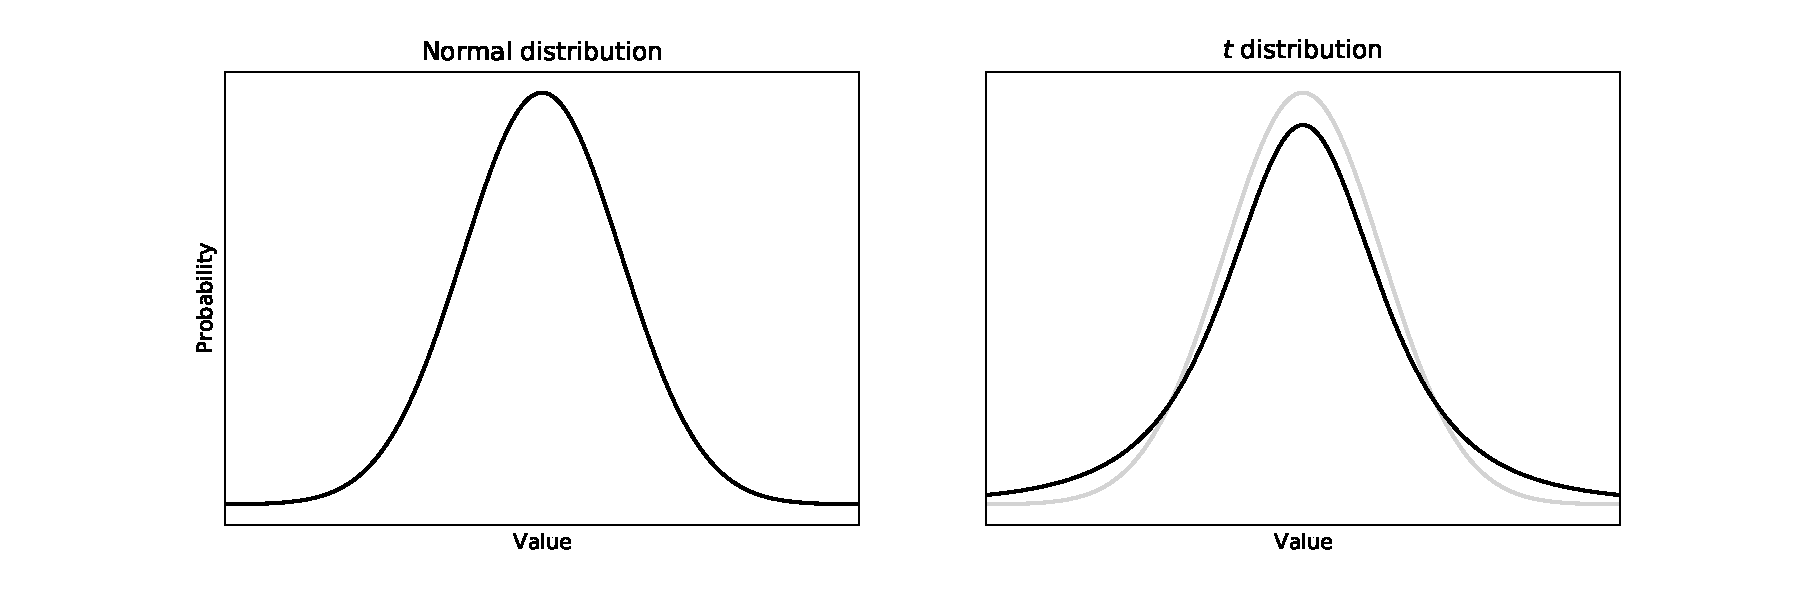
\includegraphics[width=\textwidth]{fig/distributions.pdf}
\end{frame}

\begin{frame}{A concrete example}
  \begin{itemize}
    \item Suppose you want to know if the average income in Tempe is more than \$50,000
    \item So you survey 100 people
    \item and get an average of \$52,000
    \item Does this mean the average income is more than \$50,000?
    \item If we did the survey again, would we get a different answer?
  \end{itemize}
\end{frame}

\begin{frame}{A concrete example}
  \centering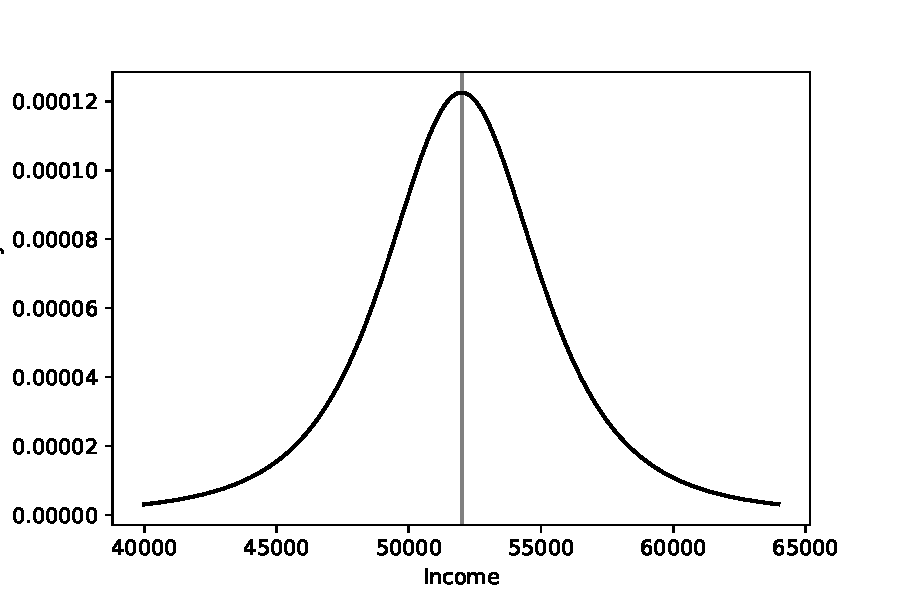
\includegraphics[width=0.7\textwidth]{fig/incdistribution.pdf}
\end{frame}

\begin{frame}{Adding some math}
  \begin{columns}
    \begin{column}{0.5\textwidth}
      \begin{itemize}
        \item The shaded area represents the probability of getting a value of \$52,000 or more if the null hypothesis is true
        \item We can integrate over this area to determine this probability, known as the $p$-value
        \item In this case it is 28\%
        \item How sure are we that the true average is more than \$50,000 now?
      \end{itemize}
    \end{column}~%
    \begin{column}{0.49\textwidth}
      \centering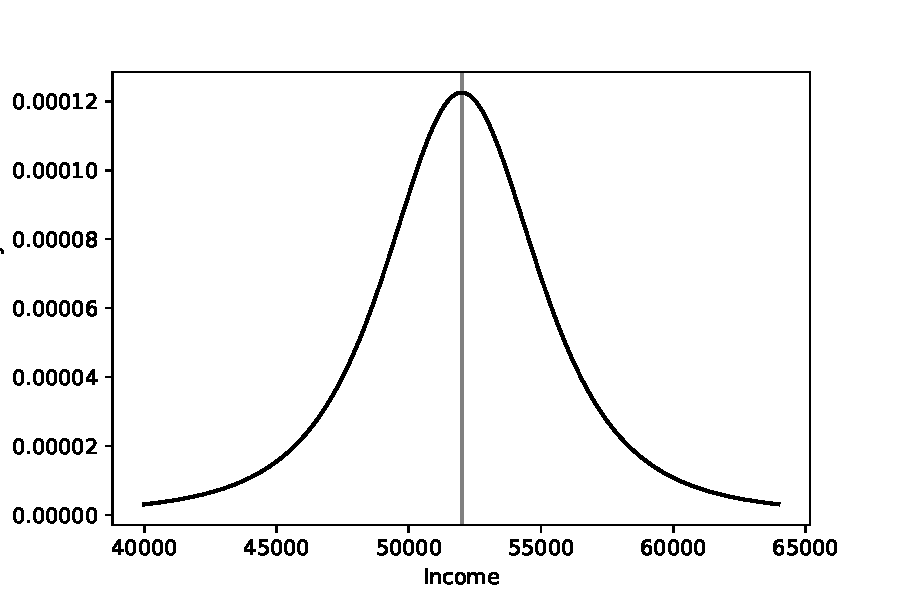
\includegraphics[width=\textwidth]{fig/incdistribution.pdf}
    \end{column}
  \end{columns}
\end{frame}

\begin{frame}{Adding some math}
  \begin{columns}
    \begin{column}{0.5\textwidth}
      \begin{itemize}
        \item A hypothesis test compares the $p$-value with a \emph{critical value}
        \item This critical value is often 0.05, but 0.1 and 0.01 are also used
        \item If the $p$-value is less than the critical value, we reject the null hypothesis and accept the alternative hypothesis
        \item Can we reject the null hypothesis in this example, with a critical value of 0.05?
        \item Which critical values are more conservative?
      \end{itemize}
    \end{column}~%
    \begin{column}{0.49\textwidth}
      \centering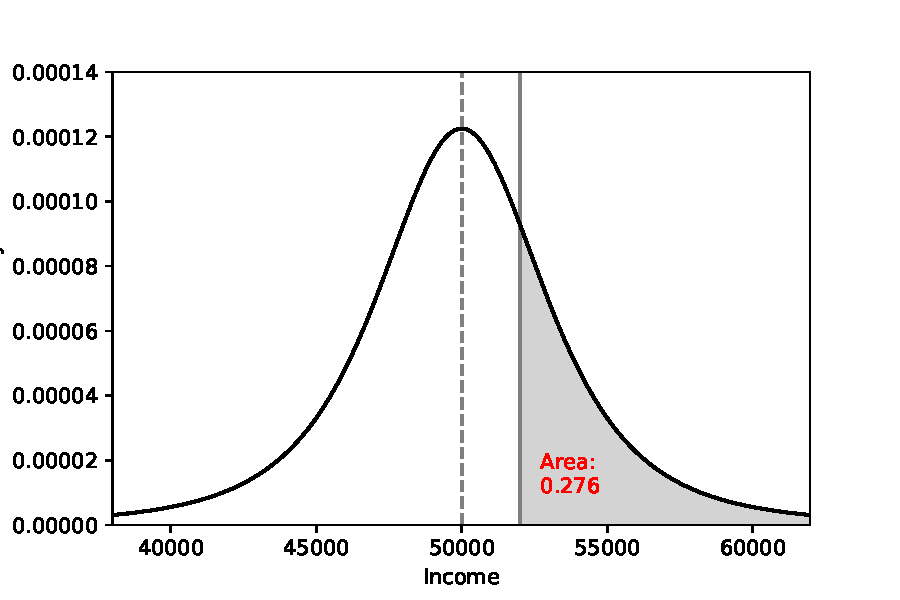
\includegraphics[width=\textwidth]{fig/incdistribution_area.pdf}
    \end{column}
  \end{columns}
\end{frame}

\begin{frame}{Aside: William Gosset and the Student's $t$ distribution}
  \begin{columns}
    \begin{column}{0.65\textwidth}
      \begin{itemize}
        \item The $t$ distribution was devised by William Gosset
        \item Gosset published under the pseudonym \textit{Student} because he couldn't publish under his own name at the request of his employer
        \onslide<2->{\item ...Guinness Brewing
          \item ...which was developing statistics to gain an edge in the beer industry}
      \end{itemize}
    \end{column}~%
    \begin{column}{0.44\textwidth}
      \begin{overprint}
        \only<1>{\centering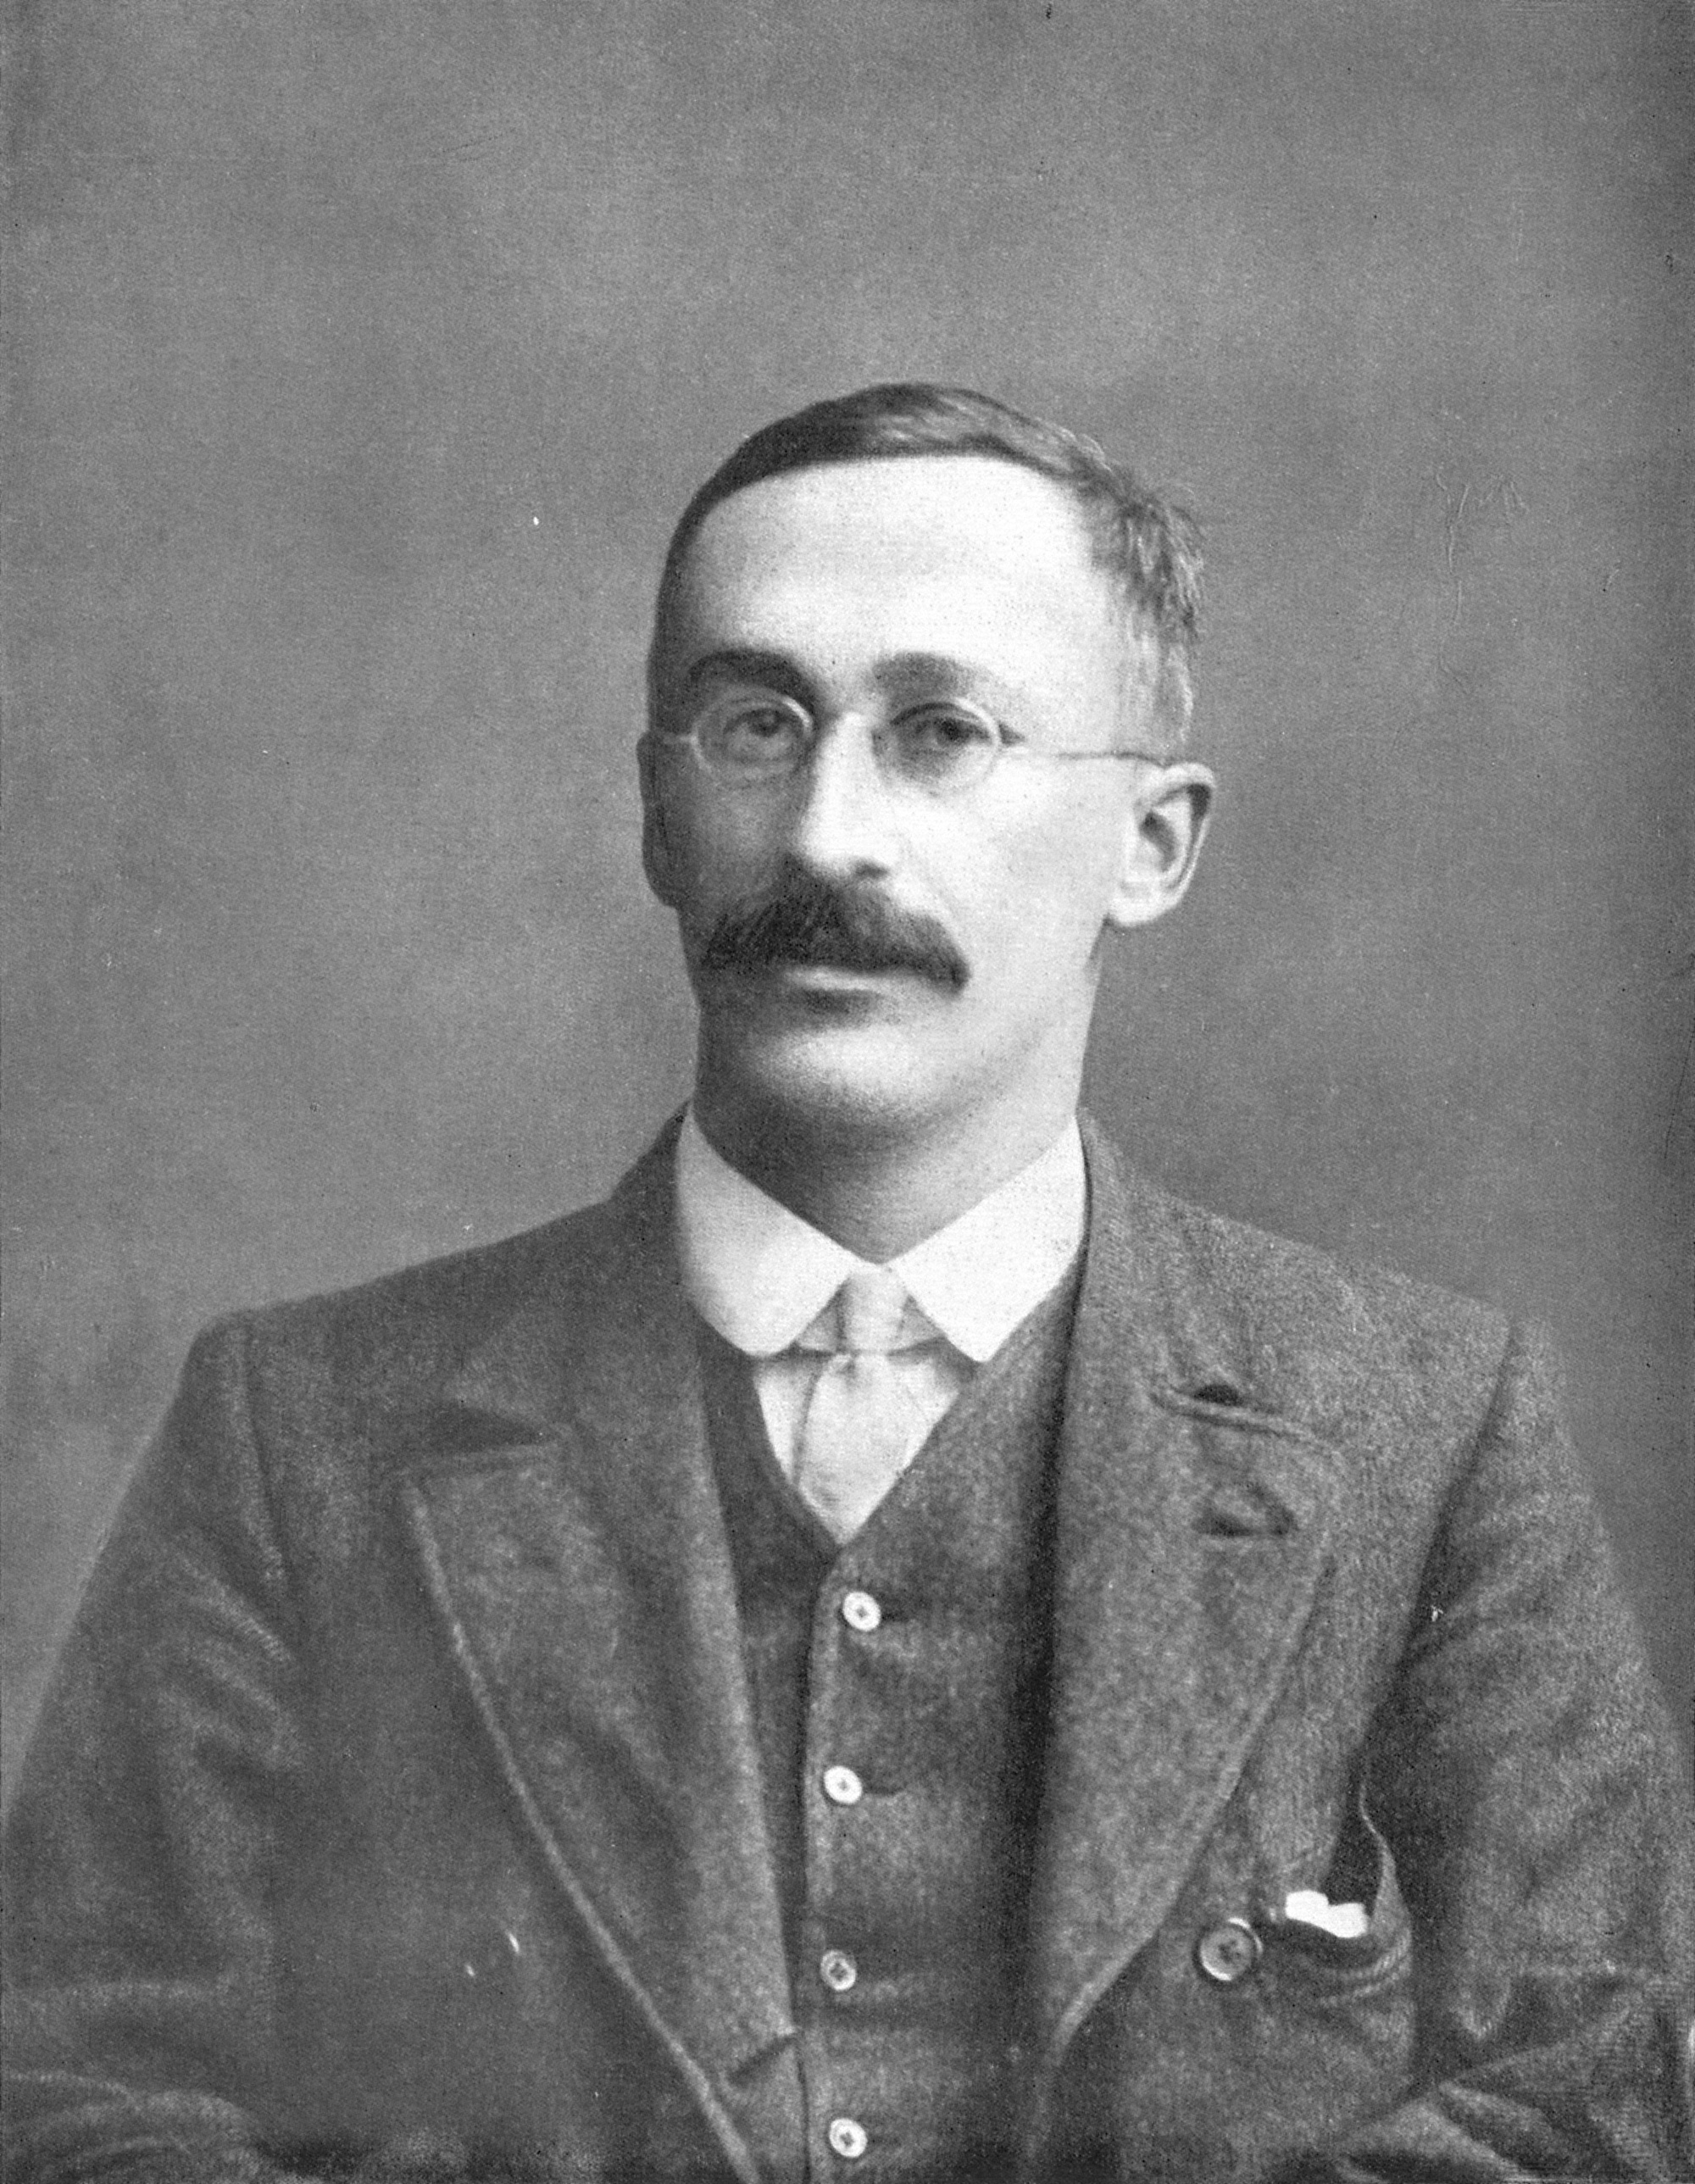
\includegraphics[width=0.7\textwidth]{William_Sealy_Gosset.jpg}}
        \only<2->{
\includegraphics[width=0.7\textwidth]{guiness.jpg}\\{\scriptsize\copyright~Malingering on Flickr, CC BY-NC-ND}}
      \end{overprint}
    \end{column}
  \end{columns}
\end{frame}

\begin{frame}{Hypothesis tests of regression coefficients}
  \begin{itemize}
    \item We can put \textit{anything} in the model and get an estimated coefficient
    \item But how do we know if this coefficient is real or due to the specific sample we're using?
    \pause\item ...with a hypothesis test
  \end{itemize}
\end{frame}

\begin{frame}{Hypothesis tests of regression coefficients}
  \begin{tabular}{lrrrrrr}
  \toprule
  {} &  Coefficient &  Std. err. &  $t$-value &  $p$-value &  95\% Conf. &  Int. \\
  \midrule
  Constant           &        -1253 &       3091 &     -0.405 &      0.685 &      -7341 &  4834 \\
  Income (thousands) &          79 &         17 &      4.593 &      0.000 &         45 &   112 \\
  Number of vehicles &         4249 &        909 &      4.674 &      0.000 &       2458 &  6039 \\
  \textcolor{red}{Day of week}        &          \textcolor{red}{272} &       \textcolor{red}{ 513} &      \textcolor{red}{0.531} &      \textcolor{red}{0.596} &       \textcolor{red}{-739} & \textcolor{red}{ 1284} \\
  \bottomrule
  \end{tabular}
  \begin{tabular}{lclc}
  Dependent variable & \multicolumn{3}{l}{Annual vehicle miles traveled} \\
  $R^2$ & 0.19 & Adjusted $R^2$ & 0.18 \\
  Sample size & 250 && \\
  \end{tabular}\\
  \tiny\citenhts
\end{frame}

\begin{frame}{Hypothesis tests of regression coefficients}
  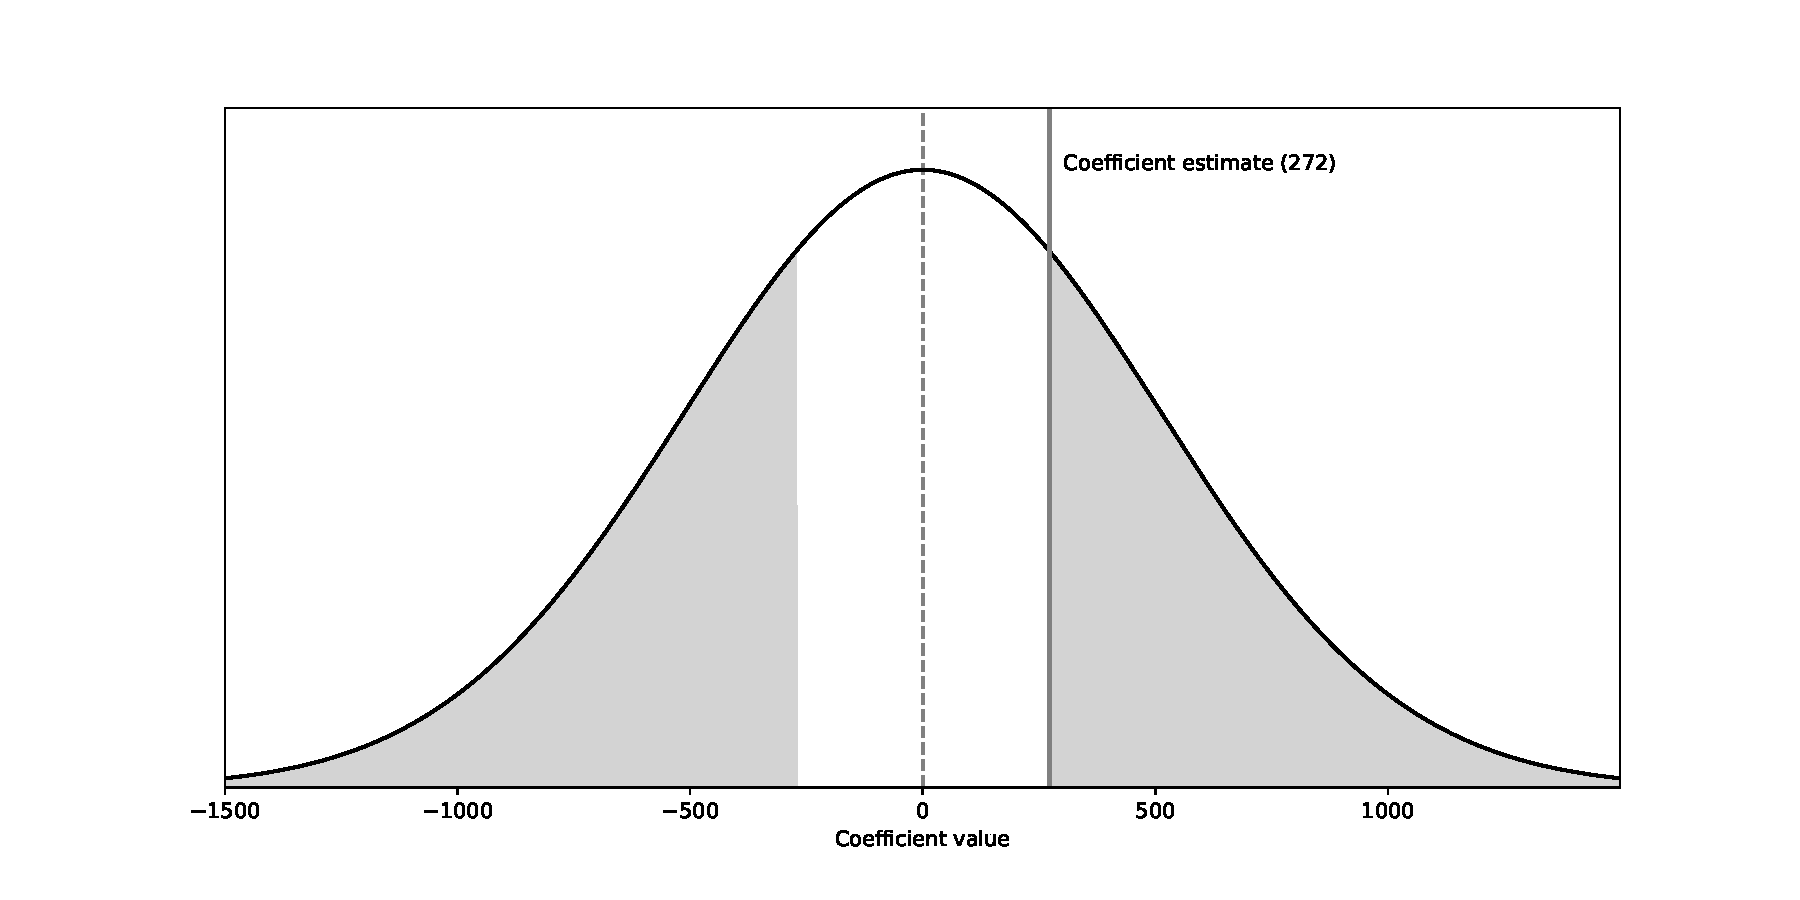
\includegraphics[width=\textwidth]{fig/coeftest.pdf}
\end{frame}

\begin{frame}{Hypothesis tests of regression coefficients}
  \begin{tabular}{lrrrrrr}
  \toprule
  {} &  Coefficient &  Std. err. &  $t$-value &  $p$-value &  95\% Conf. &  Int. \\
  \midrule
  Constant           &        -1253 &       3091 &     -0.405 &      0.685 &      -7341 &  4834 \\
  Income (thousands) &           79 &         17 &      4.593 &      0.000 &         45 &   112 \\
  Number of vehicles &         4249 &        909 &      4.674 &      0.000 &       2458 &  6039 \\
  Day of week        &          272 &        513 &      0.531 &      \tikzmark{dowp}0.596 &       -739 &  1284 \\
  \bottomrule
  \end{tabular}
  \begin{tabular}{lclc}
  Dependent variable & \multicolumn{3}{l}{Annual vehicle miles traveled} \\
  $R^2$ & 0.19 & Adjusted $R^2$ & 0.18 \\
  Sample size & 250 && \\
  \end{tabular}

  \begin{tikzpicture}[overlay,remember picture]
    \draw[red] ([xshift=1.4em, yshift=0.5ex] pic cs:dowp) ellipse (2em and 1.5ex);
  \end{tikzpicture}
\end{frame}

\begin{frame}{Standard errors, t-scores, and z-scores}
  \begin{itemize}
    \item Not every paper reports a $p$-value
    \item Some report standard errors, $t$-scores, or $z$-scores instead
    \begin{itemize}
      \item These all tell us the same information---how unlikely the observed coefficient would be if the null hypothesis were true
    \end{itemize}
    \item Standard error is the spread of the sampling distribution for the hypothesis test
    \item $t$/$z$ score is the number of standard errors between 0 and the coefficient
  \end{itemize}
\end{frame}

\begin{frame}{Standard errors, t-scores, and z-scores}
  \only<1>{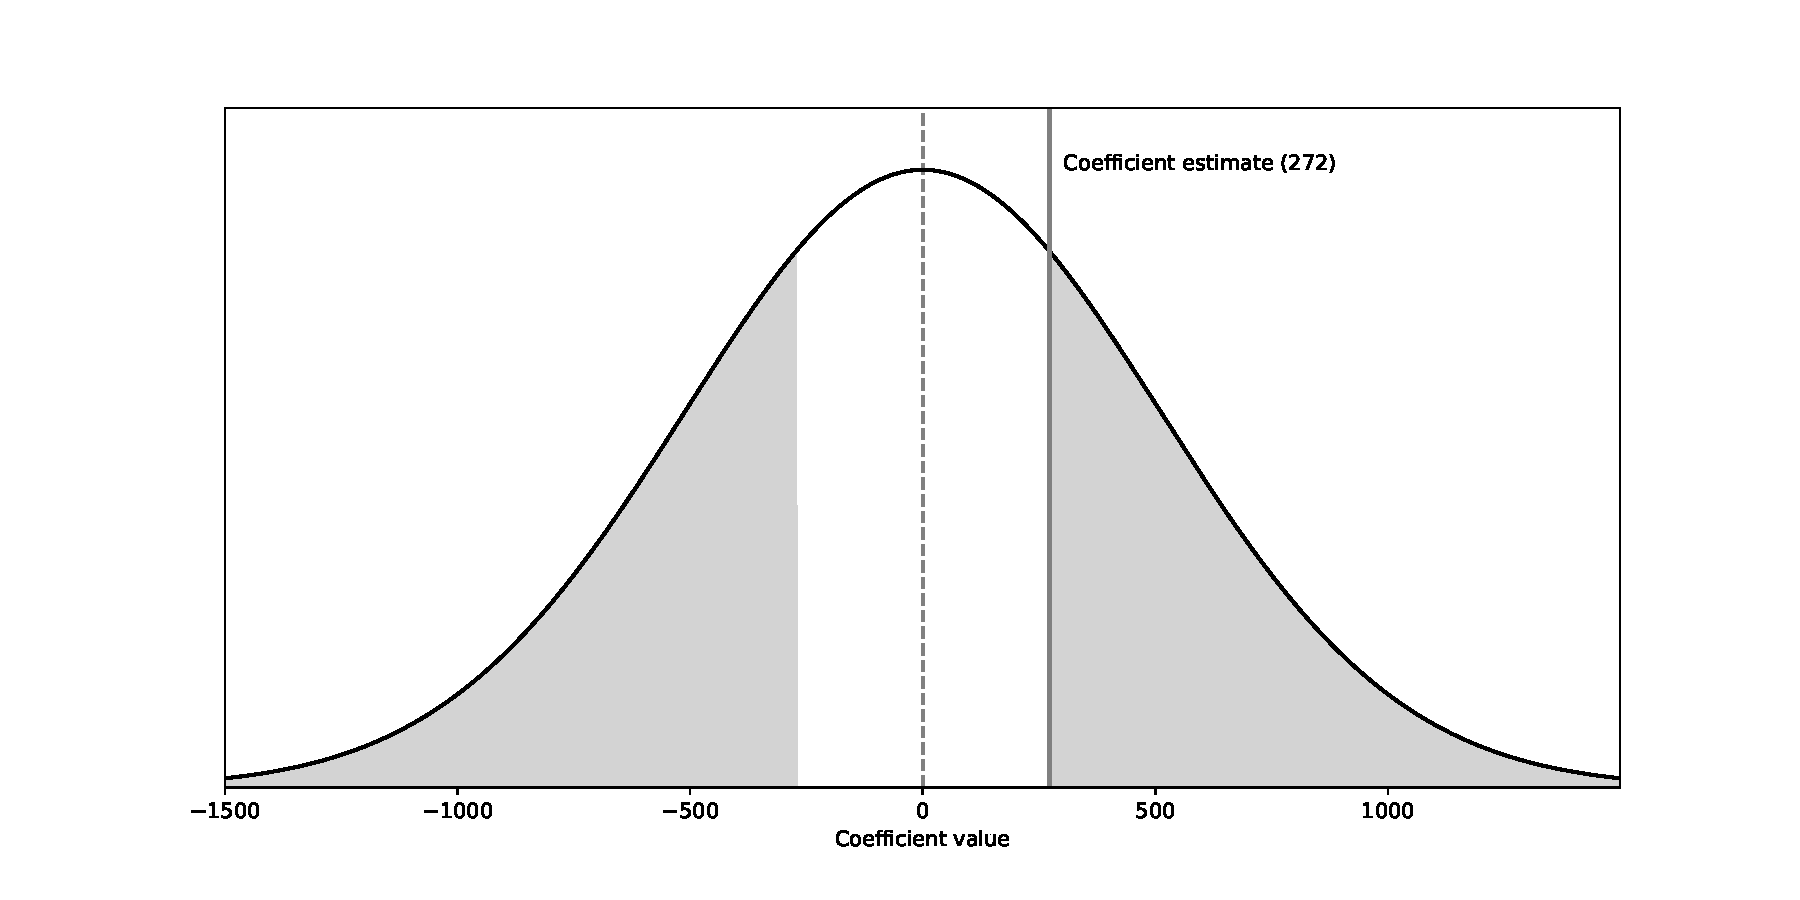
\includegraphics[width=\textwidth]{fig/coeftest.pdf}}
  \only<2>{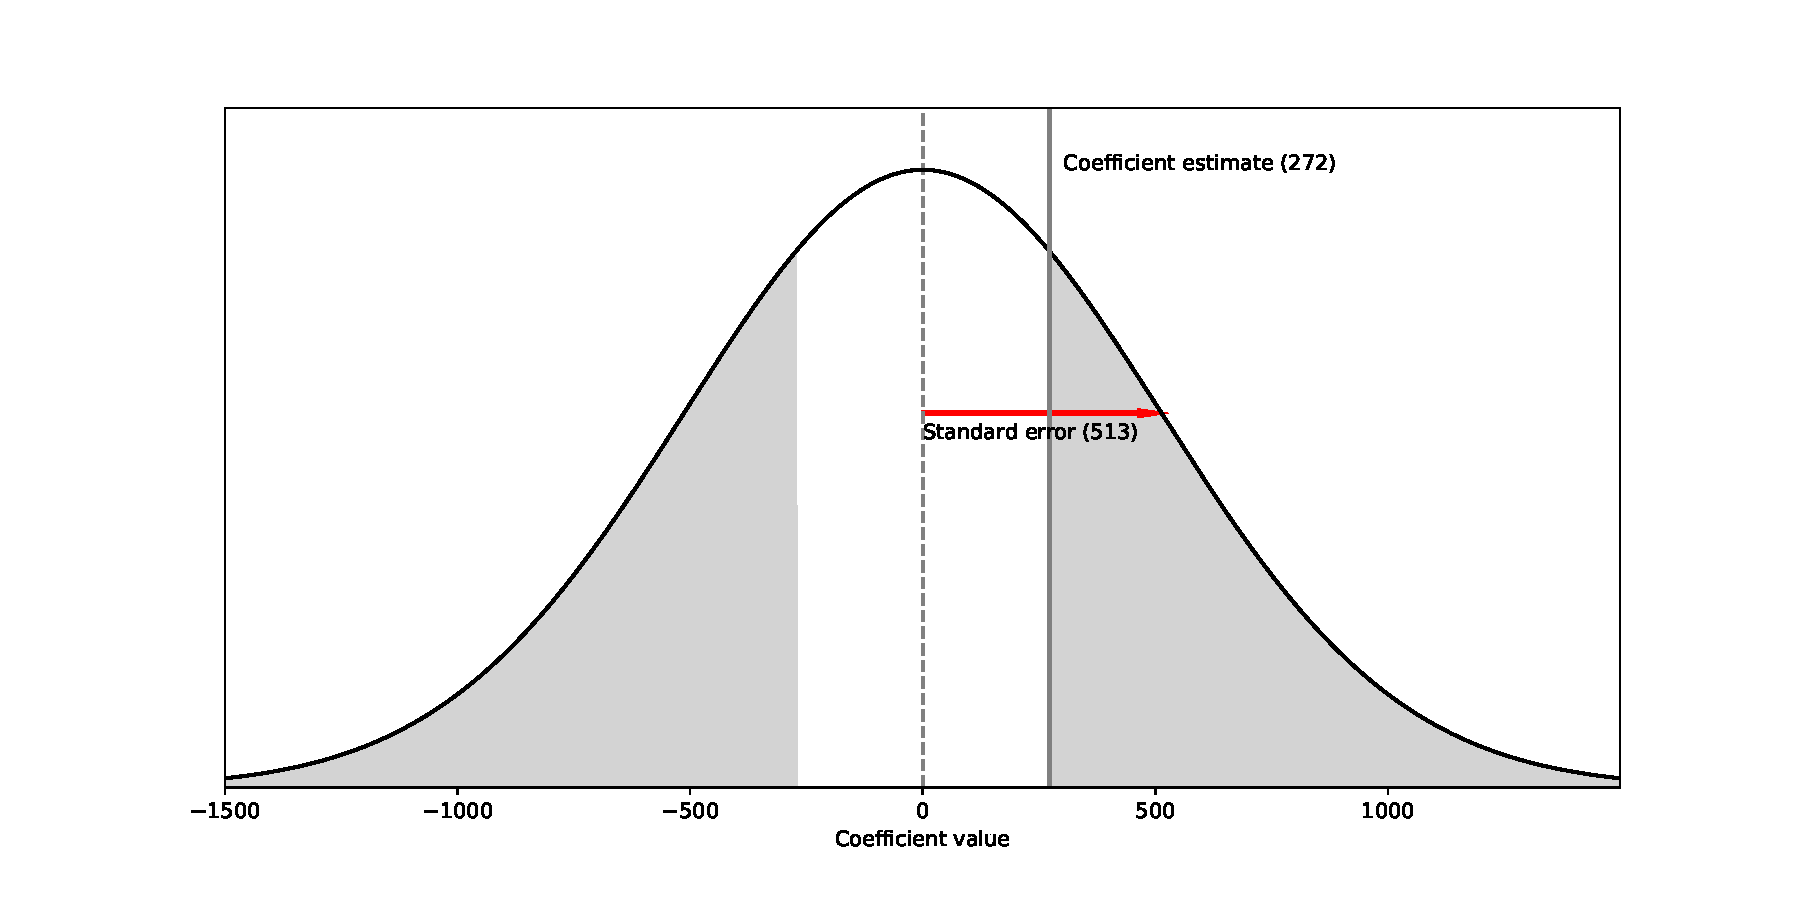
\includegraphics[width=\textwidth]{fig/coeftest_se.pdf}}
  \only<3>{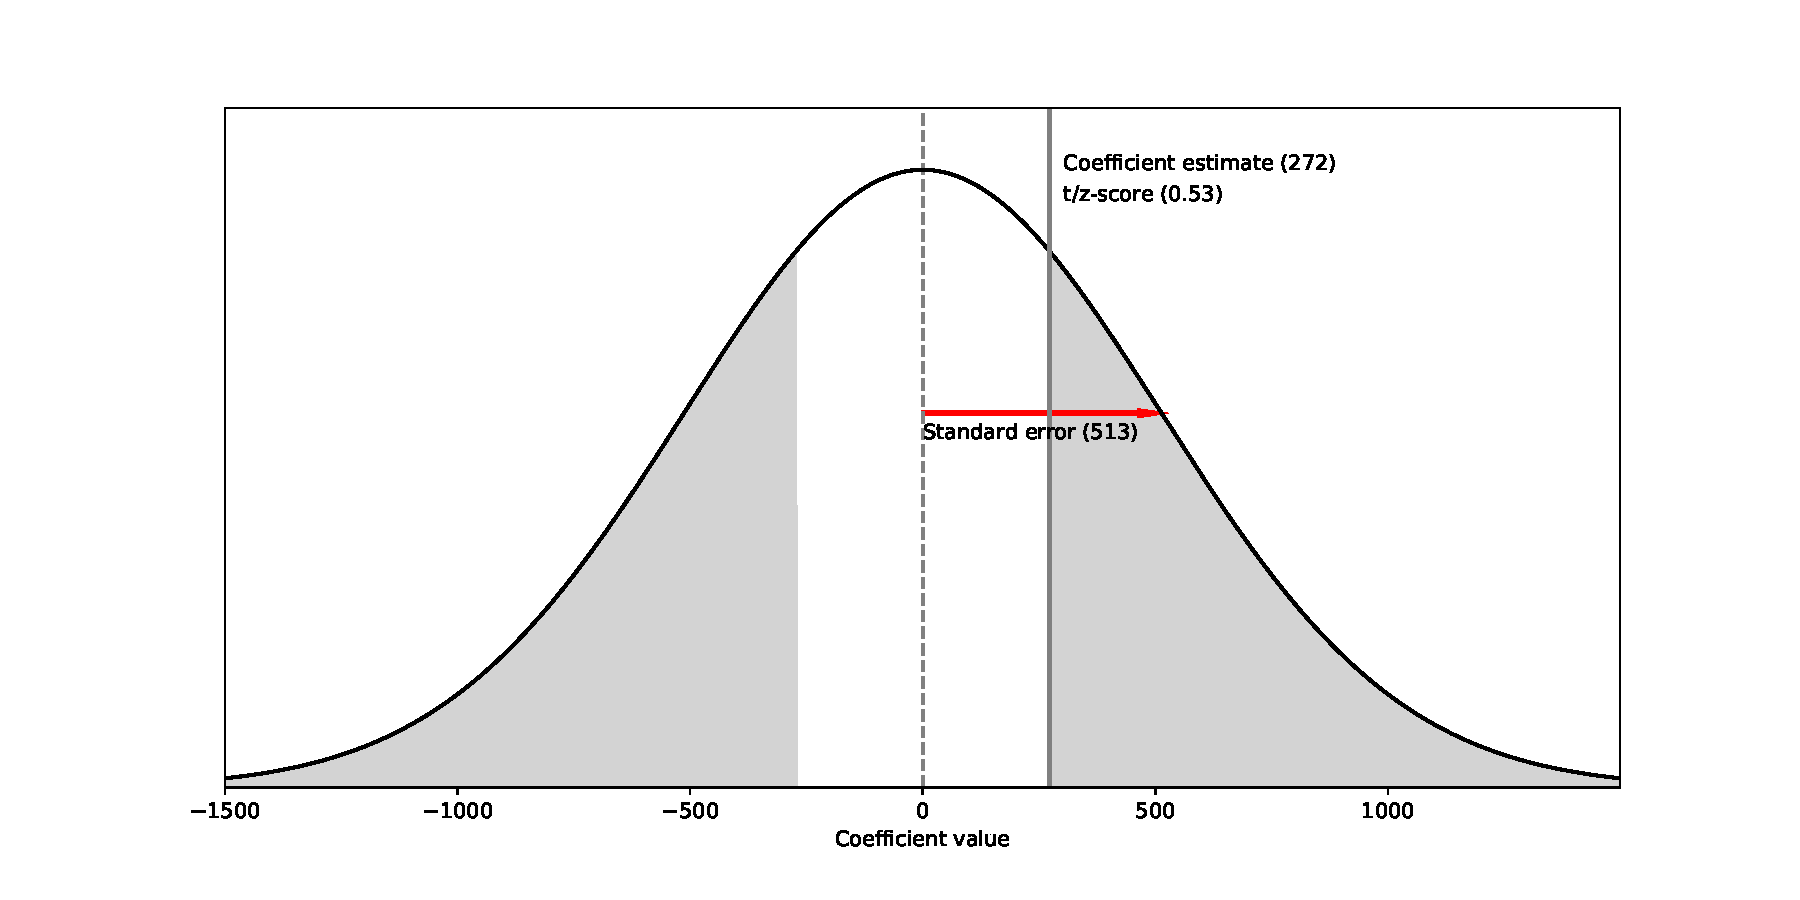
\includegraphics[width=\textwidth]{fig/coeftest_t.pdf}}
\end{frame}

\begin{frame}{Multiple testing bias}
    \begin{itemize}
      \item With a single hypothesis test, there is a small chance that we will reject the null hypothesis when it is true
      \item With many hypothesis tests, this effect compounds
      \item This can be used to $p$-hack: testing many different relationships to find one that is significant
    \end{itemize}
\end{frame}

\begin{frame}[plain]
  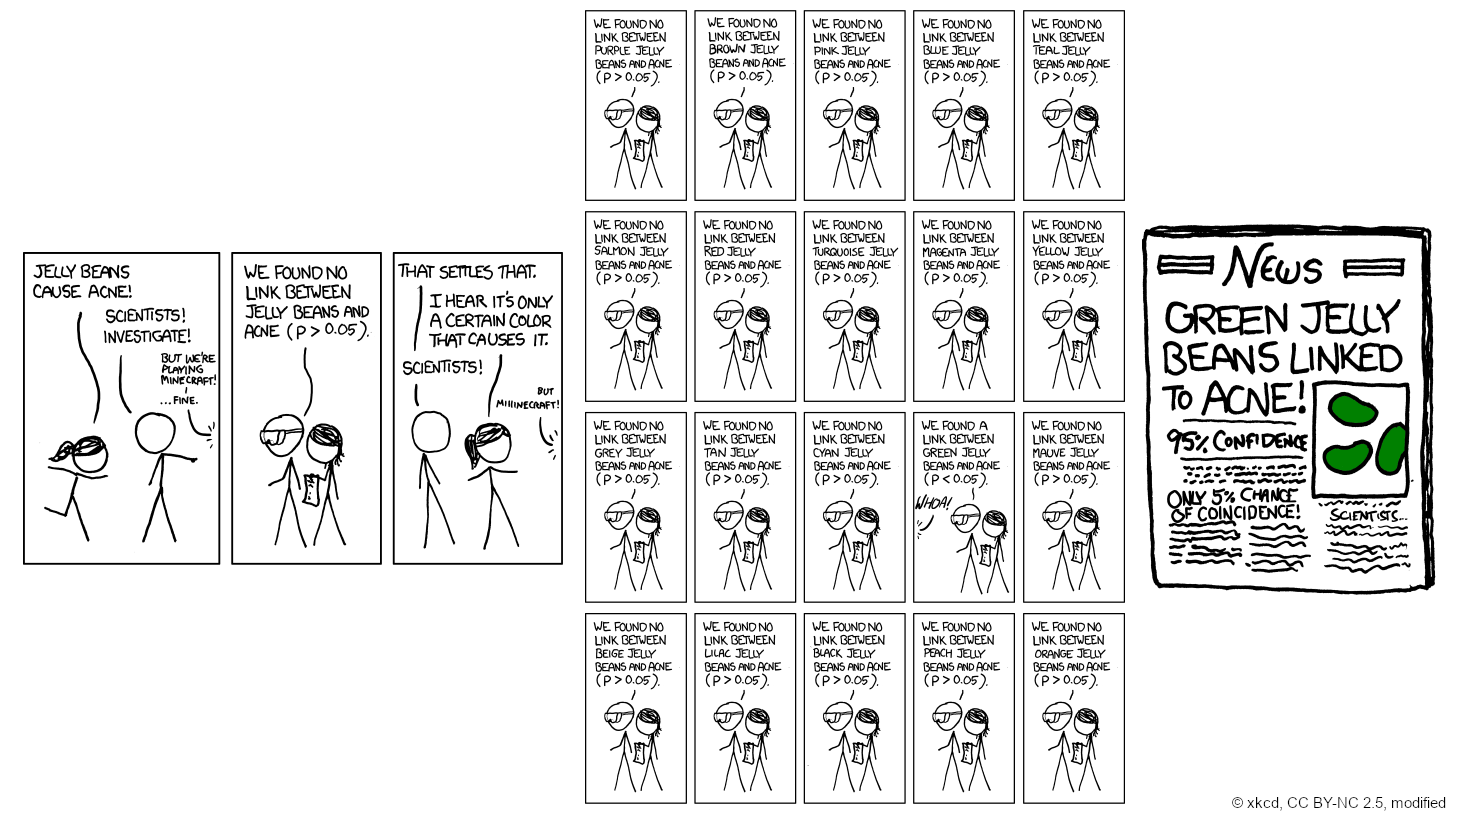
\includegraphics[width=\textwidth]{xkcd_significant.png}
\end{frame}

\begin{frame}{Multiple testing bias in regression}
  \begin{columns}
    \begin{column}{0.65\textwidth}
      \begin{itemize}
        \item Multiple testing is a particular concern in regression
        \item ...because there are so many hypothesis tests
        \item This can result in intentional or unintentional \emph{p-hacking}
        \item It is particularly a concern when authors have tested many different model forms
        \only<2>{\item Exercise: \url{https://projects.fivethirtyeight.com/p-hacking/}}
      \end{itemize}
    \end{column}~%
    \begin{column}{0.34\textwidth}
      
\includegraphics[width=\textwidth]{img/phacking-lastweek.png}\\
      {\tiny \copyright~HBO/Last Week Tonight}
    \end{column}
  \end{columns}
\end{frame}

\begin{frame}{Exclusion of insignificant variables and stepwise selection}
  \begin{itemize}
    \item Two common methods raise particular concern about multiple testing
    \item Many papers \emph{exclude insignificant variables} from their final models
    \begin{itemize}
      \item Can bias the remaining coefficients because important control variables may be excluded
    \end{itemize}
    \item \emph{Stepwise selection} selects variable for the model one at a time based on their significance
    \begin{itemize}
      \item ``[S]tepwise methods tend to capitalize outrageously on sampling error'' \autocite{thompson_stepwise_1995}
      \item i.e. stepwise selection is likely to include many variables that are significant by chance
    \end{itemize}
    \item Both of these techniques were considered \emph{state of the art} at some point, and their shortcomings have become apparent more recently
  \end{itemize}
\end{frame}

\begin{frame}{Non-sampling error}
  \begin{itemize}
    \item Non-sampling error occurs when the sample is not representative
    \item Surveying graduate students at ASU would not give you a good idea of the average income in Tempe
    \item Can also occur when people do not respond to your survey
    \item Non-sampling error is part of the concern about the Census citizenship question
  \end{itemize}
\end{frame}

\begin{frame}{Confidence intervals}
  \begin{itemize}
    \item Alternative to hypothesis tests
    \item A confidence interval is a range around the coefficient that is x\% likely to contain the true coefficient
    \begin{itemize}
      \item Usually 95\%
    \end{itemize}
    \item Does not require a null hypothesis
  \end{itemize}
\end{frame}

\begin{frame}{Confidence intervals}
  \only<1>{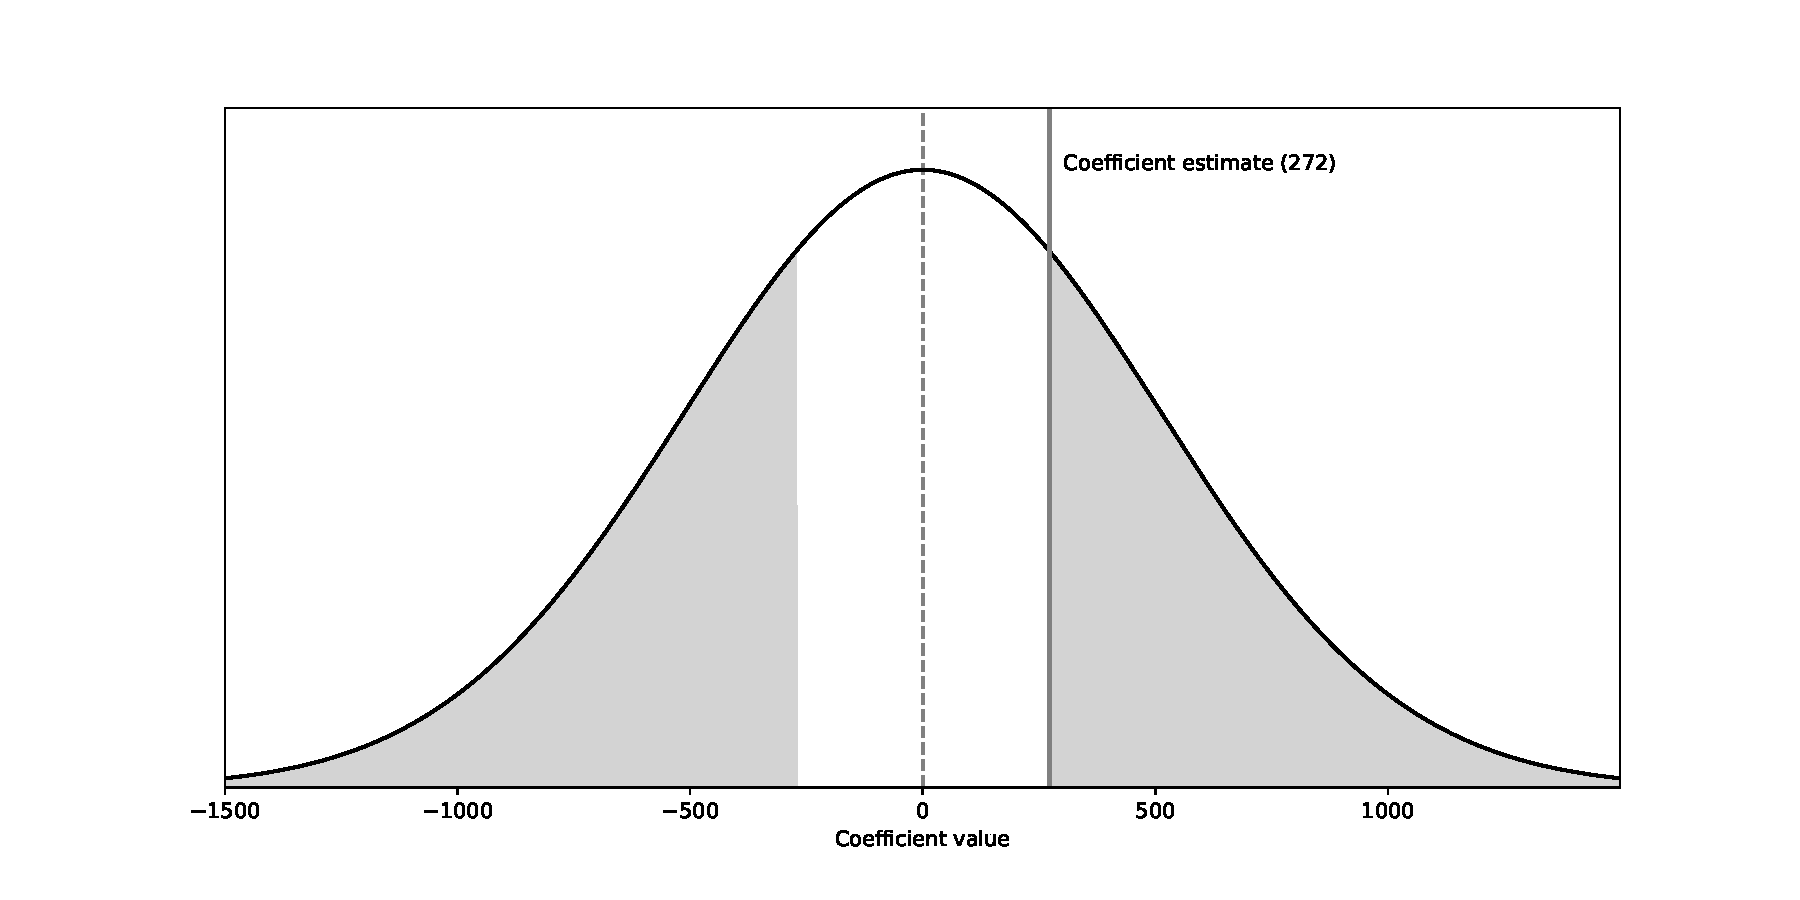
\includegraphics[width=\textwidth]{fig/coeftest.pdf}}
  \only<2>{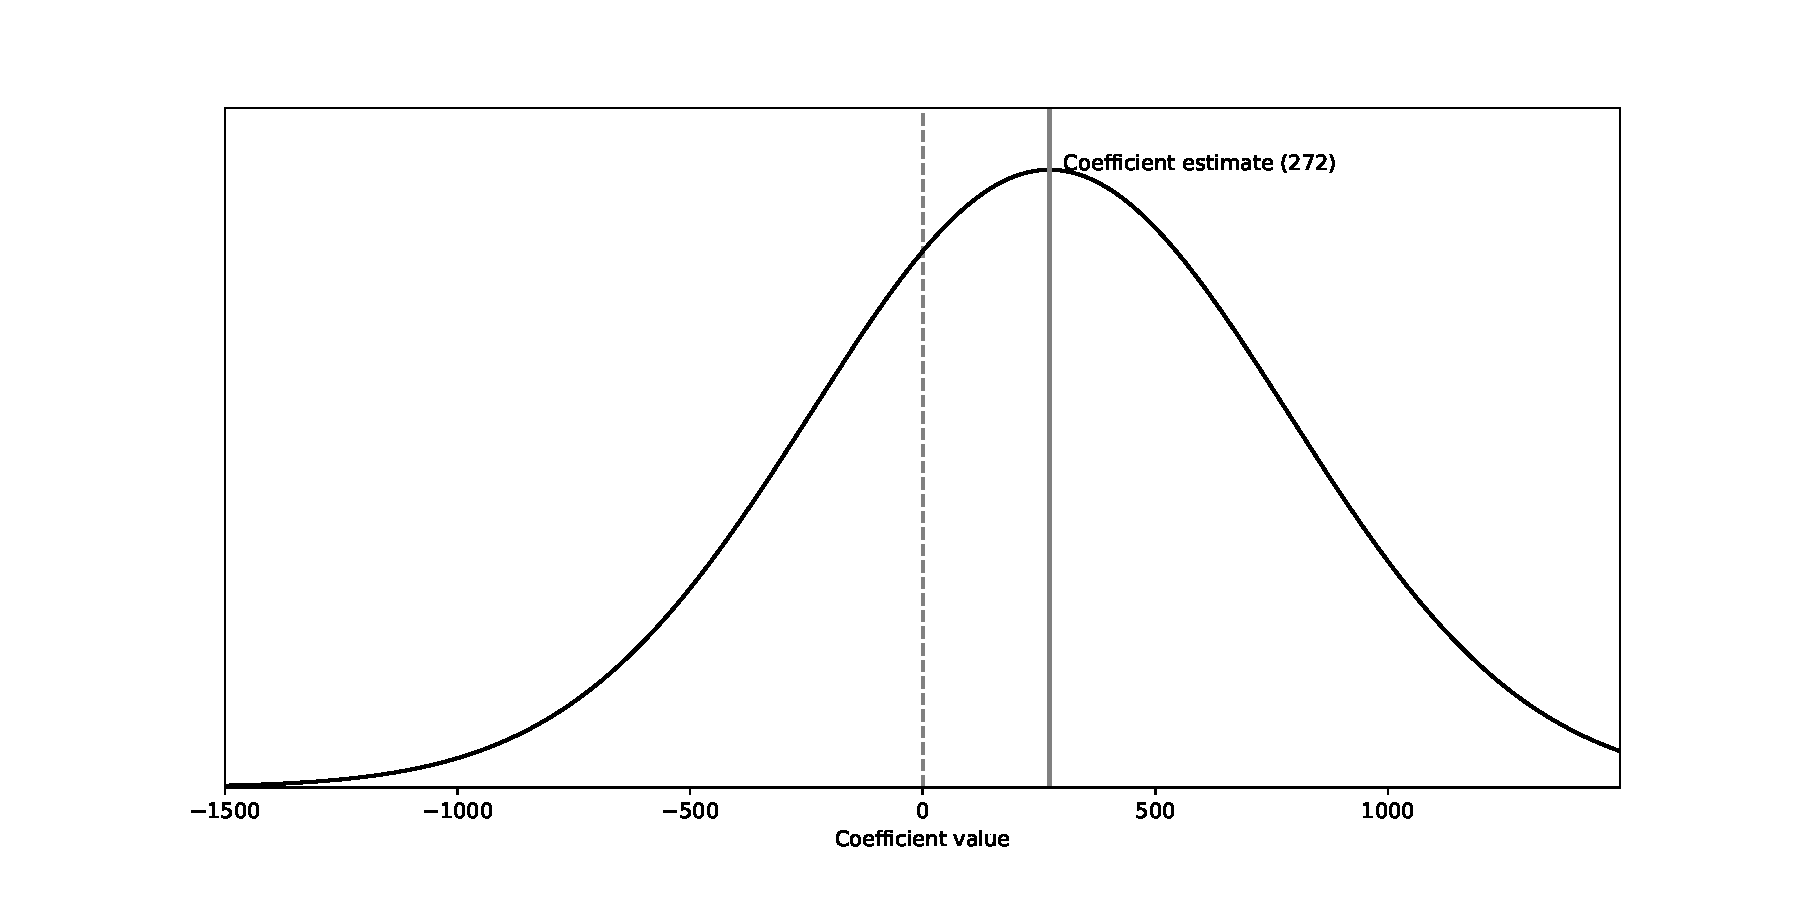
\includegraphics[width=\textwidth]{fig/confint.pdf}}
  \only<3>{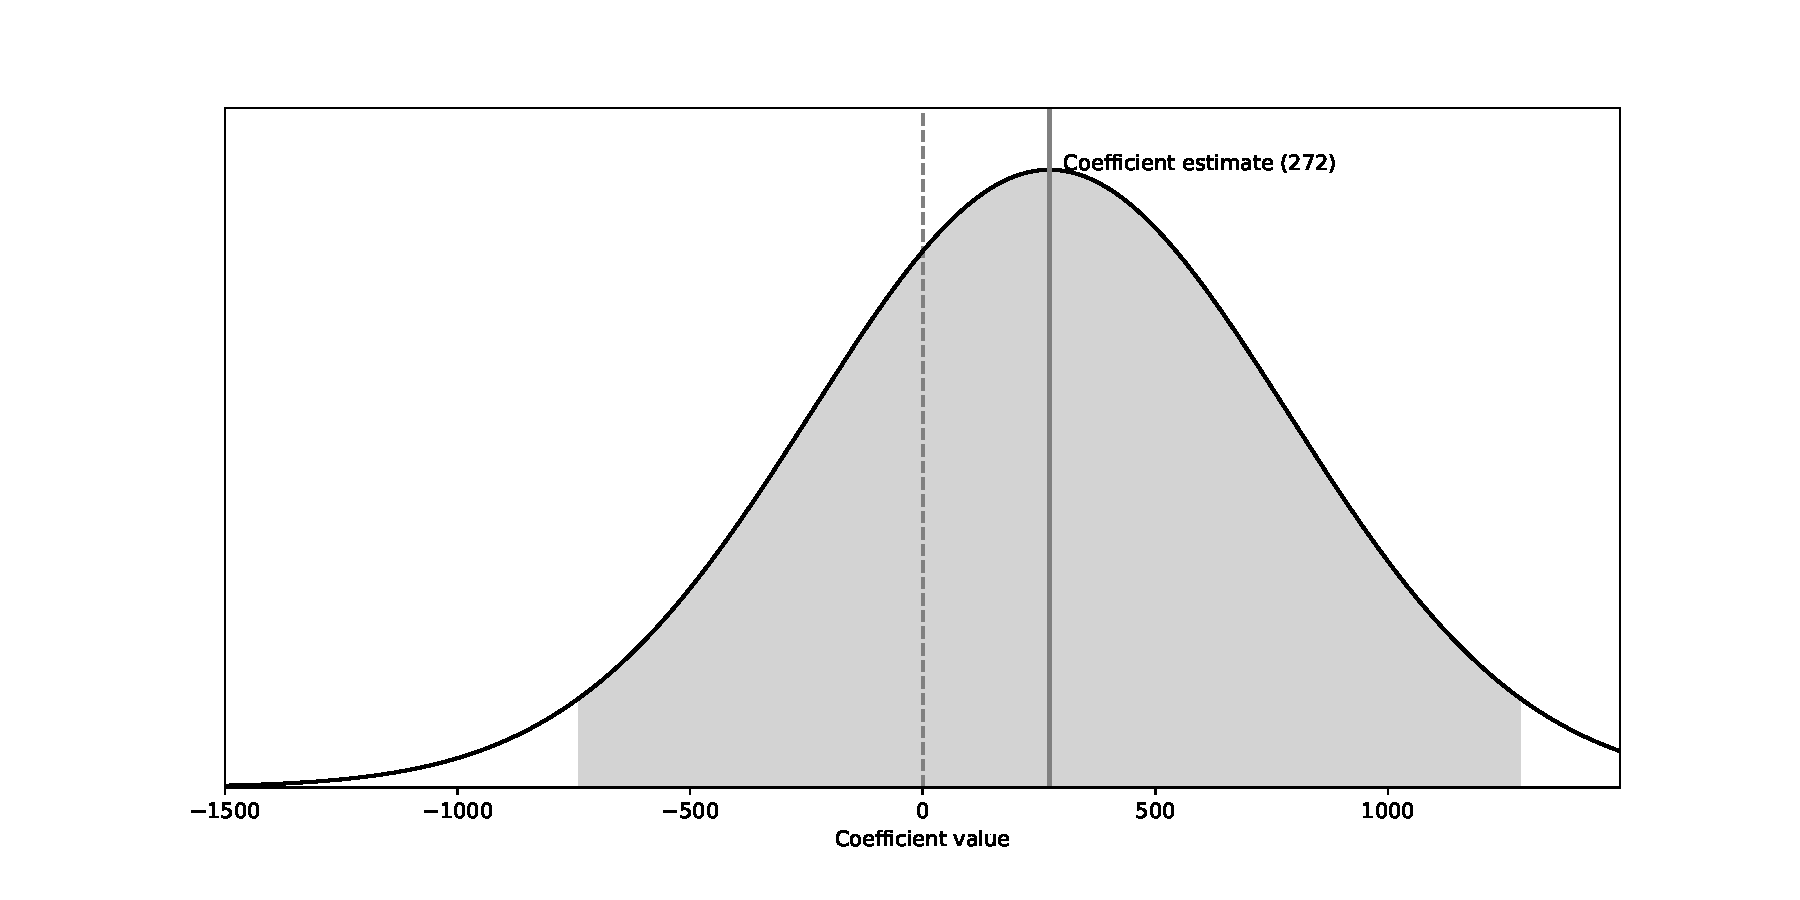
\includegraphics[width=\textwidth]{fig/confint_filled.pdf}}
\end{frame}
